%%******************************************************************************
%%
%% pesqbib.tex
%%
%%******************************************************************************
%%
%% Title......: Introduction
%%
%% Author.....: GSCAR-DFKI
%%
%% Started....: Nov 2013
%%
%% Emails.....: renan028@gmail.com
%%
%% Address....: Universidade Federal do Rio de Janeiro
%%              Caixa Postal 68.504, CEP: 21.945-970
%%              Rio de Janeiro, RJ - Brasil.
%%
%%******************************************************************************


%%%%%%%%%%%%%%%%%%%%%%%%%%%%%%
%%%%%%%%%%%%%%%%%%%%%%%%%%%%%%

\subsection{Posição Angular}

O Sistema de Lifting Beam desenvolvido em aplicação semelhante de remoção e inserção de stoplogs pela empresa \textbf{HATCH} utliza atuadores elétricos independentes em cada garra, o que permite o monitoramento da abertura das garras, sendo possível saber quando há encaixe mal ou bem sucedido. O sistema em estudo a ser desenvolvido, porém, é a monitoramento de um Lifting Beam mecânico, onde as garras abrem e fecham passivamente. Por questões de restrição de projeto, não é permitido alterar a estrutura mecânica de forma que as garras sejam atuadas independentemente, mas é permitida a instrumentação do Lifting Beam com encoders, sendo possível instalá-los nas vigas das garras, a fim de medir suas posições angulares. A movimentação angular das garras durante o encaixe é conhecido e sequencial, de forma que uma simples anlálise comparativa com os dados fornecidos pelos encoders durante a execução da tarefa pode indicar se o encaixe foi mal ou bem sucedido.

\subsubsection{Encoder}
O encoder óptico é um dispositivo eletromecânico que entrega como saída um sinal elétrico proporcional à posição angular do eixo acoplado. O eixo é acoplado mecanicamente a um disco opaco e marcado em sua superfície por segmentos (ver figura~\ref{encoder_1}).

\begin{figure}[H]
    \centering
    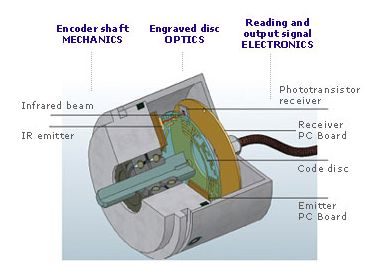
\includegraphics[width=0.5\columnwidth]{figs/encoder/1.jpg}
    \caption{Sistema interno de um encoder.}
    \label{encoder_1}
\end{figure}

Diodos emissores de luz infravermelha alcança os receptores através das fendas do disco. O sinal analógico é criado, amplificado, convertido em digital e transmitido ao processador.

Além dos requisitos básicos do projeto, como submersibilidade e resistência a choque e vibração, as principais características a serem avaliadas neste projeto para a escolha de um encoder são: modo de operação incremental ou absoluto, multi-voltas ou não, interface de comunicação, resolução e tensão de operação.

 \subsubsection{Conclusão de análise técnica}
A pesquisa mostrou ampla aplicação de encoders para a aplicação e é esperado que seja possível identificar encaixe mal ou bem sucedido com sua utielização. A instalação do encoder na viga da garra pescadora não é mecanicamente complexa e não resultará em alteração permanente da estrutura.


Os fornecedores para encoders que atendem aos requisitos de projeto pesquisados são: Hohner, IFM, Pepperl-Fuchs e Rotary Encoder Solutions. O modelo selecionado, após ampla análise entre fornecedores, é o
modelo Encoder RM9000 Absoluto com interface CAN, multi-voltas que apresenta a configuração necessária para a aplicação e o menor custo para o projeto dentro os modelos analisados. 
(figura~\ref{encoder_1})

SUBXWD	Hohner	Hohner Brasil	R$ 3.248,91
AR63	Rotary Encoder Solutions	-	R$ 2.949,61
CVS42H	Pepperl-Fuchs	Pepperl-Fuchs Brasil	R$ 2.586,46
RM9000	IFM	IFM Brasil	R$ 1.298,69

\begin{center}
    \begin{tabular}{| l | l | l | l | }
    \hline
	{\bf Modelo} 	& 	{\bf Fabricante} 	&		{\bf Distribuidor}	&	{\bf Preço} \\  \hline
	SUBXWD&			Hohner&					Hohner Brasil&			 3.248,91 R{\$} \\  \hline
	AR63&			Rotary Encoder Solutions	&	-&					2.949,61 R{\$} \\  \hline
	CVS42H&			Pepperl-Fuchs&			Pepperl-Fuchs Brasil&	2.586,46 R{\$} \\  \hline
	RM9000&			IFM&						IFM Brasil&			1.298,69 R{\$} \\ \hline
\hline 
\end{tabular}
\end{center}

\begin{figure}[H]
    \centering
    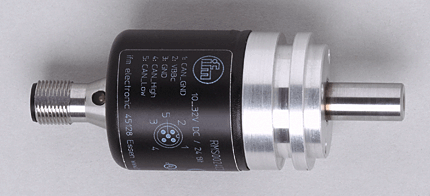
\includegraphics[width=0.4\columnwidth]{figs/encoder/1.png}
    \caption{Encoder do fornecerdor IFM}
    \label{encoder_1}
\end{figure}

